\chapter{Conflicting Paradigms}
Numerous programming paradigms exist for even more general programming languages. Each of them come with different perks and offer different perspectives for a problem. Different programming paradigms, however don't necessarily exclude each other. Languages like \textit{Lisp} or \textit{Scala} for example both combine functional and object oriented programming.\\
This thesis will specifically concentrate on \textit{Object Oriented Programming} (OOP) and \textit{Data Oriented Design} (DoD). Whether or not data oriented design is even to be considered a programming paradigm is debatable \mcp{fabian}{1}, however its fundamental ideas (specifically concerning data layout) conflict with those of existing paradigms like OOP, so for the sake of consistency in this manner of comparison, we will call it that way.\\ 
Depending on the domain, certain programmers will have different answers to the question which of both should be preferred. Each party will make compelling arguments to why their choice is mandatory. This is because those paradigms (partially) solve different problems and therefore offer dissenting perspectives on problems and their respective solutions for them.
To understand why \textit{Object Oriented Programming} and \textit{Data Oriented Design} are rather cannibalistic to each other, we need to first have a look to what they are trying to solve, independently.

\section{Object Oriented Programming / AOS}\label{OOP}
Starting with punch cards, each iteration of new programming generations provided new forms of abstraction for programmers, be it control flow statements, type systems, data structures like native arrays. When machine code started to simplify operations, FORTRAN partly introduced portability as early as 1957; LISP introduced symbolic processing and automated memory management until finally Simula/67 introduced objects in the 1960s \mc{louden}\mc{hopl}.
Object Oriented Programming could not be called popular until the 1970s or 1980s, when Stroustrup created C++. Originally OOP was meant to be the way to go for creating graphics based applications  \mc{about_oop}. This makes sense, since tree like data structures (GUIs), containing entities with shared behavior can easily be described through polymorphism.\\
OOP shines, whenever the problem to be modeled can be abstracted to one or more base classes, that define shared state and/or behavior. Even though some languages allow for a subclass to "\textit{exclude variables and/or methods which would otherwise have been inherited from the superclass(es)}" \mcp{what_is_oop}{4}.\\
OOP quickly established and rooted itself in the industry without solely being used on graphics applications. This is due to the fact, that it represents a world model, we are taught since elementary school. We are familiar with \textit{is-a} relations ever since we learned that despite dissenting traits, both Labradors and Pugs are dogs. Arguably abstraction is one of - if not - the most important disciplines in programming \mcp{ghezzi}{5}. Since programs oftentimes try to model real life information, OOP delivers an easy to grasp, quick-to-learn approach to do so. That is also the reason, why there are so many OOP programmers around the world. Without trying to evaluate whether or not OOP's way of abstraction is superior to DoD, it is undoubtedly the more prominent one, especially for virtually any other profession than a programmer/computer scientist \reffigp{lang_ratings}.
\begin{figure}[!htbp]
	\centering
	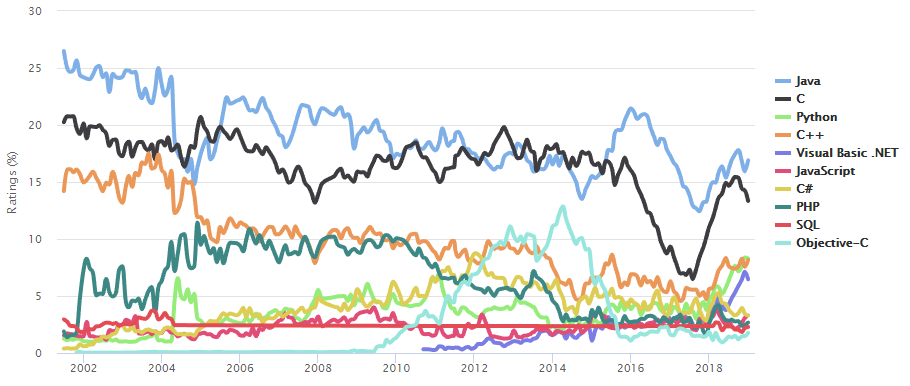
\includegraphics[width=1.0\linewidth]{PICs/lang_ratings}
	\caption{Most popular programming languages throughout the years \mcpic{lang_ratings}.}\label{lang_ratings}
\end{figure}
 This is however where OOP and modern computer architectures don't get along, so to say. OOP ovvers an elegant way to intuitively model an issue into code, but doing so it encourages us to implement our data in an inefficient way. Inefficient because creating monolithic models of our data usually lack cohesion, which means, that the classes' members tend to not be related/dependent \mc{cohesion} - at least in terms of computational order.\\
 In a home office application, juggling a few dozens of entities every other minute, this will not appear as a problem. And in this case it might be preferable to program such application in a strict object oriented way, since the development can be done fast and reliably even by a novice. On the other hand and especially in the game development industry OOP has proven to result in poorly performing software, due to inefficient data layouts. Because especially for games: data is performance \mcp{nystrom}{272}.\\
 The abbreviation \textit{AOS} stands for \textit{Array Of Structures}\mc{intel} and it describes, what usually happens with Object Oriented Programming.\\
 \begin{lstlisting}[language=C++,numbers=none,name={Example of some hierarchical POD class definitions},label={pods}]
struct Obj {				struct Human : Obj {			struct NPC : Human {
	float xyz[3];				char *name;						int mood;
	float vel[3];				int age;						};
};							};

NPC npc_arr[3];
 \end{lstlisting}
Considering the rather arbitrary C++ class definitions in \refcode{pods} the \textit{npc\_arr} will occupy memory according to \reffig{npcs_in_memory} (disregarding any \textit{padding}).
\begin{figure}[!htbp]
	\centering
	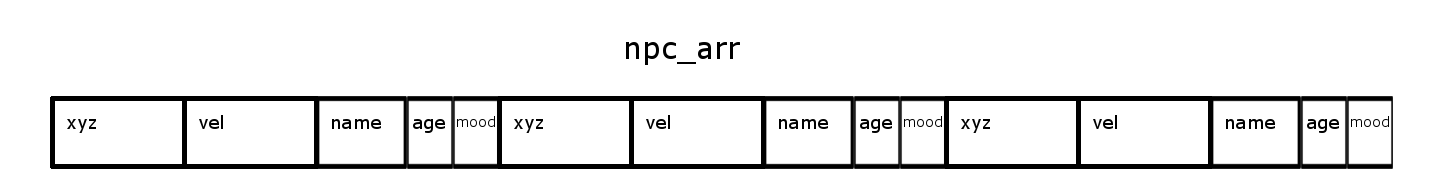
\includegraphics[width=1.0\linewidth]{PICs/npcs_in_memory}
	\caption{Visualization of how a \textit{npc\_arr} will exist in memory}\label{npcs_in_memory}
\end{figure}
This is quite literally an array of structures - hence the notation \textit{AOS}. The following sections \ref{cpu_caches} and \ref{dod} will elaborate on \textit{why} exactly this way of thinking/way of abstraction is inefficient.




\section{CPU Caches and why they don't \textit{fit} objects}\label{cpu_caches}
The data layouts typically found when programming with objects and classes, are not inefficient because they lack logic. "\textit{Each human - including students - will have positional traits}", is semantically correct. In fact it seems rather unfortunate, that modern computer architectures can't deal well with an abstraction that fits our perception of the world. But the hardware is certainly not to blame here. The problem with a monolithic class definition is much more that of common coding- or data access patterns.\\
\subsection{Common data access patterns vs. Monolithic class definitions}\label{cdap}

Numerous coding best practices teach us to write simple, modular code.
\begin{quote}
	\textit{Functions should do one thing. They should do it well. They should do it only.} \mcp{rcmartin}{35}
	
	\textit{Keep it simple and smart} (KISS principle). \mcp{niemann_kiss}{77}
	
	\textit{[...] cohesion is an important object-oriented
		software quality attribute.}\mc{cohesion}
\end{quote}
Just like we want our class definitions to share a common responsibility or task, we want the set of instructions that iterate and probably transform a set of data to be as simple and modular as possible. So usually we try to not write monolithic \textit{for-loops} handling every single aspect of a set of data.\\ For example in \reffig{npcs_in_memory} we would not want a loop that handles each and every single member of an NPC. This would not only result in a big set of instructions, that hide the individual purposes of each expression, but also make it hard to maintain/change the code. Not to mention, that different data often demands change at different times at runtime. Requirements can change quickly. Breaking up responsibilities that were coupled and forced to coexist change not so quickly.\mc{rcmartin}\\
Exemplary if \refcode{pods} was the model for a game, our game loop could at one point iterate over all the elements in the \textit{npc\_arr} to update their position and velocity for each frame. The \textit{NPC's mood} could just as well be updated frequently in a separate function, that only encompasses the information relevant for the calculation of the updated mood.
Their \textit{Human::name}s however will most likely not change so frequently - if ever - so the instructions to modify that data will most likely depend on user input and exist in yet a whole other routine. This modularization of code is commonly referred to as \textit{Separation of Concern} and has proven to improve the code's maintainability \mcp{laplante}{85}.
\textit{This} keeping the objects in some sort of set, then iterating over it for each routine, that manages a subset of the object's data, is a common access pattern that is applied on objects in OOP.\\
The interim conclusion here is, that even only for maintainability reasons, it is desirable for programmers to process logically related subsets of their data separately - but then why is the resulting software so slow compared to the same idea implemented with a \textit{Data oriented Design}?\\
The Object Oriented Programming paradigm is exactly doing what it promises - providing a sort of abstraction, that programmers can intuitively apply to their problem definition. Consequently OOP programmers quickly adapt the habit of developing against their abstraction because it is intuitive. What is lost in the process is the concern of developing against the rationale and thinking about how it interacts with the hardware. \textit{This} is probably the fundamental difference between OOP and DoD.\\
So whats our hardware's deal? Why do objects don't get along with it. Why can't we have super high speed machinery, that makes hardware concerns obsolete? Why can't we have anything nice?

\subsection{A brief history of memory}
To answer \refsec{cdap}'s concluding question: We do have high speed memory units at hand we just can't afford them. Modern computer systems rely on a variety of different memory units each differing in access latency and other properties. The intention behind this complex hierarchy of memory layers is obviously speed and is the result of an evolving cost-benefit calculation.
\begin{quote}
	\textit{The task the computer designer faces is [...] design a computer to maximize
		performance while staying within cost[...].}\mcp{hennessy}{8}
\end{quote}

Originally
\begin{quote}
	\textit{memory access latency and instruction execution latency were on roughly equal footing. [...] register-based instructions could execute in two to four cycles, and a main memory access also took roughly four cycles.}\mcp{gregory}{189}
\end{quote}
This proportion changed significantly. While it is relatively cheap to produce high speed CPUs the same is not true for memory units. So whats happening, is that today's PCs/consoles are equipped with CPUs that are way faster than the greater parts of their available memory units. Due to increasing tick rates and \textit{Instruction Pipelining} what used to be ~four cycle RAM reads are now several hundred cycles. Not Because RAM became slower - the opposite is the case - but because CPUs became that much faster in relation.
This trend was thoroughly observed and documented by John L. Hennessy and David A. Patterson \reffigp{cpu_memory_gap}.\\
\begin{figure}[!htbp]
	\centering
	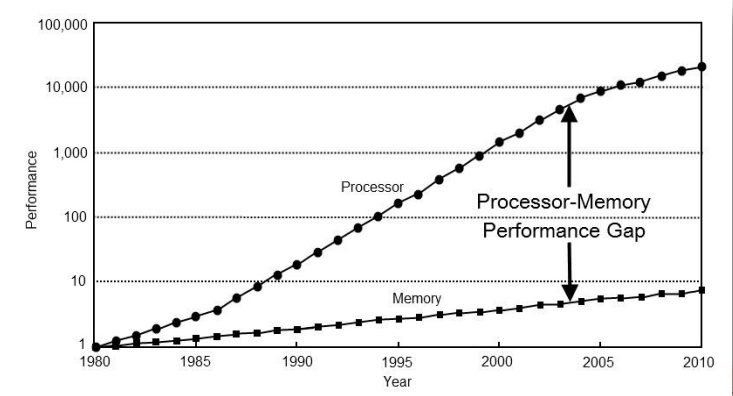
\includegraphics[width=0.7\linewidth]{PICs/cpu_memory_gap}
	\caption{"\textit{\textbf{Starting with 1980 performance as a baseline, the gap in performance
			between memory and processors is plotted over time}.
			Note that the vertical axis
			must be on a logarithmic scale to record the size of the processor-DRAM performance
			gap. The memory baseline is 64 KB DRAM in 1980, with a 1.07 per year performance
			improvement in latency (see Figure 5.13 on page 313). The processor line assumes a
			1.25 improvement per year until 1986, and a 1.52 improvement until 2004, and a 1.20
			improvement thereafter}" \mcppic{hennessy}{289}}\label{cpu_memory_gap}
\end{figure}\\
To solve the issue of ever diverging CPU/memory performances (commonly referred to as the \textit{memory gap \mc{gregory}}), specifically to reduce the latency of references to main memory, smaller but significantly faster (and more expensive) memory units are placed between the CPU and the main memory. These modules are called \textit{Caches} - first named by C.J. Conti \mc{conti} in 1969. Originally cache technology was mentioned as \textit{buffers}\mc{cragon}. Not considering their complex, modern modalities and policies this is a fitting notation.\\
The basic idea behind a fast buffer interconnected between the CPU and the main memory is to create local copies of referenced data-chunks, in order to provide faster access on subsequent calls to the same \textit{AU} (Adressable Unit) as well as the ones deemed likely to be accessed soon \mcp{gregory}{191}. This principle originated in the work on \textit{Virtual Memory} \mcp{cragon}{15} and is today much more sophisticated.\\
So we actually do use high speed memory in our common computer architecture, we just don't have lots of it.

\subsection{Cache modules and types}
In today's PCs/consoles typically each CPU core has its own hierarchy of cache modules \reffigp{cache_layout}.
\begin{figure}[!htbp]
	\centering
	\includegraphics[width=0.4\linewidth]{PICs/cachelayout}
	\caption{Exemplary, simplified model of a CPU core and its several cache modules \mcppic{Drepper}{15}}\label{cache_layout}
\end{figure}
Closest to the core (on-chip) is the \textit{L1} (Level 1) cache. Accessing an AU in the  Intel® Core™ i7 Processor's L1 cache for example is almost as fast as accessing it in the very CPU's register - ~4 cycles (2.1 to 1.2 ns) \mc{levinthal}. For reference access to main RAM "\textit{can take on the order of 500 cycles[...]"} \mcp{gregory}{189}.
Another cost unrelated reason, why we don't have lots of \textit{L1 D} cache is that more memory means literally more physical space is occupied. Having more cache memory equals more \textit{cache hits} \refsecp{cpucu} but as soon as the cache won't fit on-chip anymore, there is yet again additional latency. Thats why the L1 and sometimes L2 cache modules are kept comparably small but on-chip. Other L3 and L4 caches are each bigger and slower than their preceding counterparts respectively, but for the most part share the same ideas slowly converging latency times to the common main memory RAM.\\
CPU cores can share one or more cache modules (usually starting with L2 or L3), effectively accessing the same local copies of data. This entails synchronization issues, that will be mentioned in the context of this work later on (TODO).\\
Modern cache hierarchies include data caches as well as instruction caches, usually both in an L1 cache. However there are different takes on how to implement this. Harvey G. Cragon lists \mcp{cragon}{17}:
\begin{itemize}
	\item instruction cache - holds only instructions
	\item data cache - holds only the data stream
	\item unified cache - holds both instructions and data
	\item split cache - two-cache system, one for instructions and one for data
\end{itemize}
The scope of this masters thesis will omit instruction-cache related subjects, because the upcoming attempts and techniques to achieve performance optimizations will focus on improving the data layout of a given target source code.
%local  L1 CACHE hit,                              ~4 cycles (   2.1 -  1.2 ns )
%local  L2 CACHE hit,                             ~10 cycles (   5.3 -  3.0 ns )
%local  L3 CACHE hit, line unshared               ~40 cycles (  21.4 - 12.0 ns )
%local  L3 CACHE hit, shared line in another core ~65 cycles (  34.8 - 19.5 ns )
%local  L3 CACHE hit, modified in another core    ~75 cycles (  40.2 - 22.5 ns )
%remote L3 CACHE (Ref: Fig.1 [Pg. 5])        ~100-300 cycles ( 160.7 - 30.0 ns )

\subsection{The CPUs cache utilization}\label{cpucu}
A programmer will rarely ever directly interact with a cache module (though there are mechanisms for manual prefetching/clearing). The underlying idea for it was to be transparent to the programmer. However understanding the CPUs cache utilization enables one to tailor the data layout to it, resulting in faster access, less waiting and consequently higher throughput. Among other things, this is what \textit{Data oriented Design} aims to do - developing against hardware concerns.\\
As mentioned before the basic idea of the cache is to provide local copies of data at a faster rate and prefetch data segments, that are likely to be used soon. This works by directing each main memory access to go through the cache. Main memory access means also going through virtual address translation, address and data buses and depending on the main memory, crossbar switching logic \mcp{gregory}{190}.  
Whenever the CPU requests access to a certain AU before saddling the horses and going on a journey to main memory, the cache will check whether or not the requested AU is currently present inside its buffer. If so it is referred to as a \textit{cache hit}, otherwise a \textit{cache miss}. For a modern L1 D cache this buffer, to be more specific, consists of several cache lines usually each of 64 bytes. Overall cache- and line sizes vary between different architectures but are standardized mostly due to Intel's designs.\\
Cache misses result in higher access latency and should be avoided if possible. It is however not always possible. \textit{Mark Donald Hill} describes three classifications for cache misses:
\begin{itemize}
	\item Compulsory Miss - Access to previously unreferenced data blocks. The very first data access will inevitably result in a main memory access.
	\item Conflict Miss - Due to data blocks mapping to the same cache-lines.
	\item Capacity Miss - Due to the cache's finite capacity. Lots of data access will eventually displace older/less-used entries in the cache (depending on Replacement policies).
\end{itemize}
The simplest and least efficient implementation to determine a cache \textit{hit/miss} is to iterate each cache line comparing fitting criteria. To prevent this nowadays caches implement a certain associativity technique. This way each individual physical main memory address can be mapped to one or more specific cache lines. Doing so addresses are converted to and managed by metadata consisting of: \mcp{gregory}{193}
\begin{itemize}
	\item Offset - Offset to the actual referenced Byte inside the cache line.
	\item Cache Line Index - Which cache line/s would hold the AU.
	\item Tag - Which cache sized block in main memory holds the original data.
\end{itemize}
In the case that each physical main memory address, has exactly one counterpart it is called a \textit{direct-mapped} cache \mcp{gregory}{194}. In this case since the cache can by far not encompass the whole extend of the main memory, a lot of physical addresses will be mapped to the very same cache line, effectively extruding each other out of the cache when accessed. This is called \textit{eviction} and in unlucky cases will behave like all references are cache misses \mcp{cragon}{97}. To prevent this modern caches map a physical address to \textit{n} cache lines. This is called \textit{n-way associativity} - typically implemented as \textit{8-way} or \textit{16-way} caches depending on the level.\\
There is a lot more to cover about caching technologies and policies like: Replacement-/Write-/Coherency(MESI; MOESI; MESIF) policies and for further reading Harvey G. Cragon's \textit{Memory Systems and Pipelined Processors}\mc{cragon} as well as Jason Gregory's \textit{Game Engine Architecture}\mc{gregory} are highly recommended reads. However for the purpose of this work a few specifics are most interesting for us.\\
How can a data layout affect \textit{hit ratios} and reduce calls to main memory? As mentioned before there are common data access patterns in software and the caches actually accommodate us by adapting their builtin prefetching mechanisms to it, following a set of \textit{locality concepts}. Harvey G. Cragon counts three of those concepts: \mcp{cragon}{16}
\begin{itemize}
	\item \textit{Temporal locality} - Information recently referenced by a program is likely to be used again soon.
	\item \textit{Spatial locality} - Portions of the address space near the current locus of reference are likely to be referenced in the near future.
	\item \textit{Sequential locality} - A special case of spatial locality in which the address of the next will be the immediate successor of the present one.
\end{itemize}
At first glance these concepts are very straight forward, but their respective implementations for automatic hardware prefetching can be more complex than one would think. Prefetching basically means:
\begin{quote}
"\textit{[...] bringing data in the data (or mixed instruction-data) cache before it is directly accessed by a memory instruction [...].}" \mcp{chen}{610}
\end{quote}
There are however different strategies to decide which bytes should be faithfully loaded into the cache. Tien-Fu Chen and Jean-Loup Baer list two categories for prefetching strategies: \mcp{chen}{610}
\begin{itemize}
	\item \textit{Spatial} - access to current block is basis for prefetching.
	\item \textit{Temporal} - lookahead decoding of instruction stream is implied.
\end{itemize}
There are simple approaches like: whenever block \textit{i} is accessed, prefetch block \textit{i}+1, called the \textit{One Block Lookahead}; stride based approaches storing previously referenced addresses in a table and calculating a stride based on current and previous addresses; combinations of both and many more \mc{chen}.  Sometimes data is prefetched into the cache, sometimes into separate stream buffers. There are many different hardware prefetching methods to find and while data cache prefetching is considered to be more challanging \mcp{mittal}{4} it is still best practice to rely on spatial locality when modeling data to play into the cache's hand.\\
Compilers already make use of software prefetching (manual cache interaction instructions) in certain cases.
\begin{quote}
	\textit{For array-based applications, the compiler can use locality analysis to predict which dynamic references to prefetch, and loop splitting and software pipelining to schedule prefetches.} \mcp{luk}{223}
\end{quote}
So we can already deduce that for an efficient data layout it would be beneficial to rely on arrays, or more generally, concepts compilers can 'comprehend' and optimize. Also even though the concept of \textit{sequential locality} is only a special case, it is the one we can utilize best to derive adaptations for our data layout, since hardware prefetching has adapted best to it. How exactly can we convert this information into a generic set of rules/best practices, a methodology for efficiency? We don't it already exists.

\section{Data Oriented Design / SOA}\label{dod}
The whole purpose of adding abstraction layers is moving further away from the hardware mentally. This helps us to focus on constructing appropriate models for a problem \mcp{kramer}{5}. However disregarding intrinsic detail is predestined to result in poor resource utilization at that level. \textit{Data oriented Design} wants us to be fully aware of what is beneath the source code and tailor the essential resources to it. Essential resources here being our data. 
\begin{quote}
	\textit{The data-oriented design approach doesn't build the real-world problem into the code. This could be seen as a failing [...] by veteran object-oriented developers [...]. [It] gives up some of the human readability [...], but stops the machine from having to handle human concepts [...].}\mcp{fabian}{7}
\end{quote}
\subsection{OOP and bad abstraction}\label{oop_bad_abstraction}
DoD however deserves more credit than only being a performance optimization. (Wrong) abstraction not only moves us away further from the hardware, but also from the actual problem domain.\\
Even though \textit{coupling} and its avoidance are a big deal in OOP it somehow seems natural to couple the data and the problem domain. This coupling has proven to lead to the exact same problems as coupling of unrelated classes. Its hard to make changes, especially when the reason for change is modification of fundamental design choices. But not only is contextual linkage rigid to conceptual change but its also hard to operate on it only in ways that haven't been thought of initially.\\
Imagine for example a simple particle system implemented in a typically OOP manner \refcodep{particle_system}.
 \begin{lstlisting}[language=C++,numbers=none,name={OOP typical particle system implementation},label={particle_system}]
struct particle
{
	float ms_alive, lifetime_in_ms;
	float xyz[3];
	Shader *shader;
};

struct particle_system
{
	particle particles[1024];
	unsigned particles_alive;
	...
};
\end{lstlisting}
At first glance it appears to be a perfectly valid approach to make a particle system linked directly to the very particles it is supposed to manage. Each method will now operate on the particles array and just like that we can make numerous particle systems, each implicitly operating only on its own data. This is an easy to grasp concept that in terms of a particle system we could easily match with a real-world fireworks battery. While there are a few things, that can be nagged about, concerning only maintainability there is already a huge issue.\\
What about operations, that need to be applied to ALL particles? ... Why should we? When in the real world do two physically different particle systems ever interact with each other? Collision might come to mind. While it would be a lot easier to just iterate a big list of particles, we don't really care. It is still relatively easy to just check each particle system's particles against another particle system \refcodep{collision}. And we will just do this for all the particle systems we have! They probably should exist somewhere in the same context anyway.\\
 \begin{lstlisting}[language=C++,name={Example code how OOP could handle collision between different particle systems' particles},label={collision}]
void particle_system::particle_system_collision(
	particle_system *ps1,
	particle_system *ps2)
{
	for(unsigned i = 0; i < ps1->particles_alive; ++i)
	{
		particle *p1 = ps1->particles[i];
		for(unsigned o = (ps1 == ps2 ? i+1 : 0); o < ps2->particles_alive; ++o)
		{
			particle *p2 = ps2->particles[o];
			auto collision_data = sphere_collision(p1->m_xyz, p1->m_radius, p2->m_xyz, p2->m_radius);
			if(collision_data.colliding)
			{
				collide(*p1, *p2, collision_data);
			}
		}
	}
}
\end{lstlisting}
Even though \refcode{collision} has some uncomfortable specifics (especially line 8), it is still doable. The moment we start to render this particle system however we might notice that our particles look weird. Our particles' sprites make use of transparency and even though we enabled transparency in our render back-end it doesn't look right. Well the particles need to be rendered in a certain order. We have not thought of that while designing our data model. Its easy enough to sort one particle system's particles according to their distance to camera respectively, but bringing EACH particle system's particles in order?\\
Well we could write an algorithm, that has a list of particle arrays; takes each particle system's particle array; unifies them to a big dynamically allocated array; then sorts it; then returns that array so it can be rendered. Each frame. While we are at it, we will need to change our render pass, since now we don't render each particle system, but one big array of particles.\\
This is starting to get ugly really fast. We never do this stuff for a real-world fireworks battery and we feel betrayed by the abstraction we made. Ultimately we come to a point where we understand, that a real-world projection of a problem domain into source code might not be the best choice. Its definitely possible, but just doesn't \textit{fit} right. So instead of realizing overly complex solutions to make our code fit our abstraction we realize that our abstraction is obsolete and we should focus on a solution that fits our tasks. In the end data is not generic in the way it is used \mcp{fabian}{15}. Different jobs might require different solutions and OOP might be optimal for a subset of problems, but has evolved into a pattern, that is forced on domains as a go to.\\
Besides additional layers of abstraction do not equal superior usability/readability either. When using a third party library we hope the API designer provides functions that operate on data types we are already familiar with, like char pointers, instead of forcing us to learn how to use that developers self-made string class (KISS).\\\\
So arguably Object Oriented Programming is not automatically superior, neither in terms of maintainability nor performance. Actually it appears to be inferior to DoD. What does DoD do to be harder/better/faster/stronger?

\subsection{Normalization of Data}
When thinking in terms of the problem and designing against the data \textit{Richard Fabian} references relational database models as a worthy category to look up to, in his book \textit{Data-Oriented-Design: Software engineering for limited resources and short schedules}. After all a database should handle data correctly. Fabian says:
\begin{quote}
\textit{The structure of any data is a trade-off between performance, readability, maintenance, future proofing, extendibility, and reuse.} \mcp{fabian}{28}
\end{quote}
We have already seen, that the object typical data-layout makes sense in terms of readability, but fails to be maintainable and in terms of cache utilization behaves poorly. In order to peel off of the OOP abstraction pattern we want our model to be a minimal, precise representation, that abides a format, that has proven to behave well. Therefore we attempt to treat our data modeling process the way we would, when setting up a relational database. We normalize our data, according to the existing normalization stages developed by Edgar F. Codd and Raymond F. Boyce \mc{codd}. This is certainly not done because relational databases are famous for their excellent performance (they are not), but because it has proven to give advantageous insights to the data, its domain and the relations between its subsets. Dealing with the problem's domain and the underlying data eventually led to technologies like JPEG and MP3 \mcp{fabian}{47}. Understanding the data will lead to an understanding of the solution.\\
For our minimal example of a particle system, even just the first stages of normalization teaches us, that there should be no arrays of data in one element \mcp{fabian}{37} it also forces us to reconsider which data is accessed through which instance (key) and therefore whether or not there is a \textit{relation} to find \reftablep{normalized_ps}.\\
\begin{table}
	\centering
	\scalebox{0.7}{
	\begin{tabular}{@{}lllllll@{}}
	\toprule
	\textbf{particle\_id} & \textbf{shader\_id} & ms\_alive & lifetime\_in\_ms & x   & y    & z     \\ \midrule
	p0                    & s0         & 7034      & 10000            & 4.0 & 10.1 & -12.9 \\
	p1                    & s0         & 122       & 10000            & 0.5 & -8.1 & -2.6  \\
	p2                    & s0         & 4310      & 10000            & 1.1 & 7.4  & -3.0  \\
	...                   &            &           &                  &     &      &       \\
	p1024                 & s1         & 86        & 100              & 7.0 & 0.0  & 0.5   \\
	p1025                 & s1         & 44        & 100              & 3.0 & 0.0  & 0.2   \\
	... &&&&&& \\
	\bottomrule
	\end{tabular}}
\end{table}
\begin{table}[]
	\parbox{0.5\linewidth}{
		\centering
		\scalebox{0.7}{
		\begin{tabular}{@{}cll@{}}
			\toprule
			\textbf{system\_id} & particles\_alive\\ \midrule
			ps0                 & 462                   \\
			ps1					& 99				   \\ \bottomrule
		\end{tabular}}
	}	
	\parbox{0.5\linewidth}{
		\centering
		\scalebox{0.7}{
		\begin{tabular}{@{}cll@{}}
			\toprule
			\textbf{system\_id} & \textbf{particle\_id}\\ \midrule
			ps0                 & p0                   \\
			ps0                 & p1                   \\
			ps0                 & p2                   \\
			...                 &                      \\
			ps1					& p1024				   \\
			ps1					& p1025				   \\
			... & & \\ \bottomrule
		\end{tabular}}
	}

	\caption{Example excerpt of how the simple particle system could be normalized}
	\label{normalized_ps}
\end{table}
\\
We will not implement a relational database for our application but generating this model can help us realizing some things.
\begin{enumerate}
	\item particles are no longer represented block-wise inside a particle system, but are held in ONE unified table to begin with.
	\item There is tons of redundancy. Not logical but contextual. Seeing the same \textit{shader\_id} and \textit{lifetime\_in\_ms} over and over for each particle that will share a particle system certainly \textit{smells} funny. It is very important to be able to link each particle to a specific shader, but contextually this is redundant. We can see, that some things might have been coupled due to our abstraction.
	\item Instead of holding an array of particles we can just as well take its data subsets and link them against a unique key, which basically translates to each column is an array and each key is an index.
	\item Rethinking which data belongs to which entity hints at \textit{when} specific subsets are accessed and in which context (which key is used to get it).
\end{enumerate}

\subsection{Structure of Arrays}
In contrast to the previously mentioned AOS \refsecp{OOP} a \textit{Structure of Arrays} is the \textit{column-oriented database} pendant to a data layout that results in higher throughput by providing a cache friendly structure \mcp{fabian}{163}. We already know, that the hardware, specifically the cache uses certain strategies to prefetch data out of main memory \refsecp{cpucu}. Now when implementing the column-oriented approach that comes with data normalization we automatically almost perfectly conform to those hardware prefetching mechanisms. We do so by implementing columns as arrays. The original concept of an \textit{object} can now be simplified to an index, that retrieves the respective values in each column/array.
Remembering \refcode{pods}, when examining the NPC class we know that after derivation (done by the compiler) it looks like \refcode{post_deriv_npc}.
\begin{wrapfigure}[14]{l}{.35\textwidth}
\begin{lstlisting}[language=C++,name={NPC pod after derivation is done},label={post_deriv_npc}]
struct NPC 
{
	//inherited from Obj 
	float xyz[3];
	float vel[3];
	//inherited from Human
	char *name;
	int age;
	//NPC
	int mood;
};
\end{lstlisting}
\end{wrapfigure}
Accessing subsets of an instance of NPC will always result in loading at least a whole cache line. Lets assume, that the game code will iterate over the NPCs to update their positions by adding their velocity and some delta-time to their current xyz. Modern architectures mostly rely on cache lines of 64 Byte and assuming that \textit{sizeof(NPC)} is 40 Byte we can make the following assumptions. Considering the subset of data we actually want to work with on our update routine per NPC is (2 * 3 * \textit{sizeof(float)}) 24 Byte, we waste 40 - 24 = 16Byte of our cache-line per NPC. 
If we had 1000 NPCs instead of only 3 to actually compute each NPCs updated position we would load 40.000 Byte. 16.000 Byte of that would be ignored in total. The smallest common multiple of our 40 Byte NPC and our 64 Byte cache-line is 320, so over eight NPCs worth of cache-line we can count the amount of cache misses produced and extrapolate to greater numbers of NPCs \reffigp{cache_utilization_npc}.
\begin{figure}[!htbp]
	\centering
	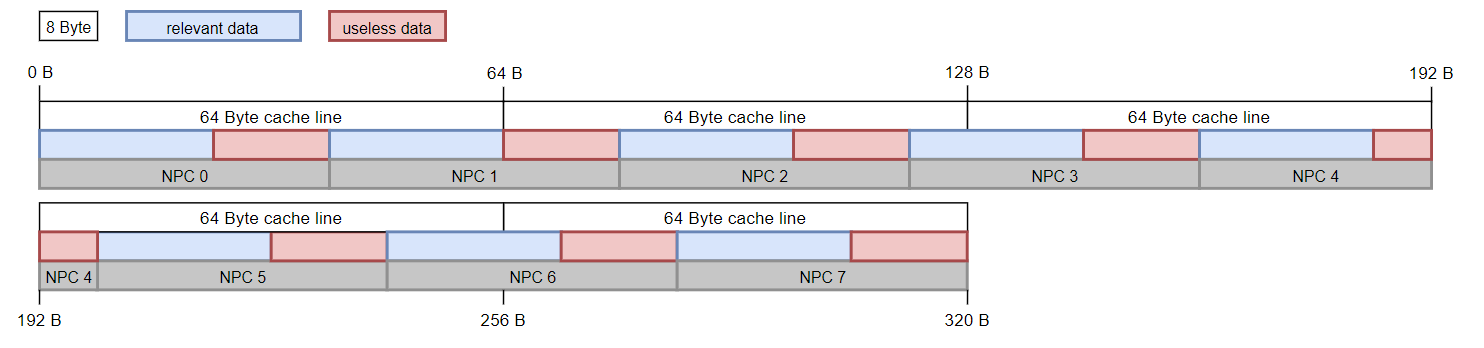
\includegraphics[width=1.0\linewidth, height=0.3\linewidth]{PICs/CacheUtilizationNPC}
	\caption{NPCs inside cache-lines, where blue is relevant data and red blocks represent unused data}\label{cache_utilization_npc}
\end{figure}
For the purpose of simplicity and demonstration we will assume that the cache will only ever prefetch to the extend of loading the complete cache-line. In reality depending on the strategy any number of lines could be prefetched asynchronously. A cache miss occurs whenever we do not find an AU inside a cache line in terms of our visual representation in \reffig{cache_utilization_npc} this means, for each cache line we can count the first occurrence of a blue block that is at least intersecting the cache-line. While \textit{NPC0} completely fits inside the first cache-line, \textit{NPC1} does not. However \textit{NPC1}'s relevant data also completely fits in the first cache-line, so accessing it's relevant data will not result in a cache miss! While accessing \textit{NPC2}'s relevant data will partly load \textit{NPC3}'s relevant data, we will only prefetch the first eight Byte of it.
\begin{lstlisting}[language=C++,name={SOA variant of the NPC},label={soa_npc}]
struct NPCs{
	float xyz[3 * NUM_ENTITIES];
	float vel[3 * NUM_ENTITIES];
	char *name[NUM_ENTITIES];
	int age[NUM_ENTITIES];
	int mood[NUM_ENTITIES];
};

NPCs npcs;

void update_npc_position(unsigned npc_id){
	float local_xyz[3];
	float local_vel[3];
	memcpy(local_xyz, npcs.xyz + npc_id * 3, sizeof(float[3]));
	memcpy(local_vel, npcs.vel + npc_id * 3, sizeof(float[3]));
	local_xyz[0] += local_vel[0] * delta_t;
	local_xyz[1] += local_vel[1] * delta_t;
	local_xyz[2] += local_vel[2] * delta_t;
	memcpy(npcs.xyz + npc_id * 3, local_xyz, sizeof(float[3]));
}
\end{lstlisting}
The remnant will be loaded separately from main memory, yet this will result in completely loading \textit{NPC4}'s relevant data.\\
Continuing this we will count five cache misses and foregoing from 320 loaded Bytes this process will repeat. When eight NPCs result in five cache-misses for 1000 NPCs we will count $1000 npc = \frac{5 * 1000}{8} cms = 625 cms
$ for the position update routines (where \textit{cms} are cache misses).\\\\
After normalizing the \textit{Obj}; \textit{Human}; \textit{NPC} thematic and implementing it in a SOA manner it could look like \refcode{soa_npc}. What used to be individual class members are now columns/arrays, accessed by a key - the \textit{npc\_id}. From now on both reads to \textit{xyz} and \textit{vel} will fill a cacheline worth of relevant data, respectively. A single cache-line now holds up to five positions or velocities. This doesn't prevent our data from overlapping in terms of cache-lines. This can be solved by adjusting the data's \textit{alignment}. Since this will be used in the prototypical implementation it will be explained in TODO REF-SECTION, for now we could assume, that we align and pad our \textit{float[3]} blocks of data to our cache-lines in a way that each cache-line holds exactly five of those relevant entities \reffigp{cache_utilization_soa}.
\begin{figure}[!htbp]
	\centering
	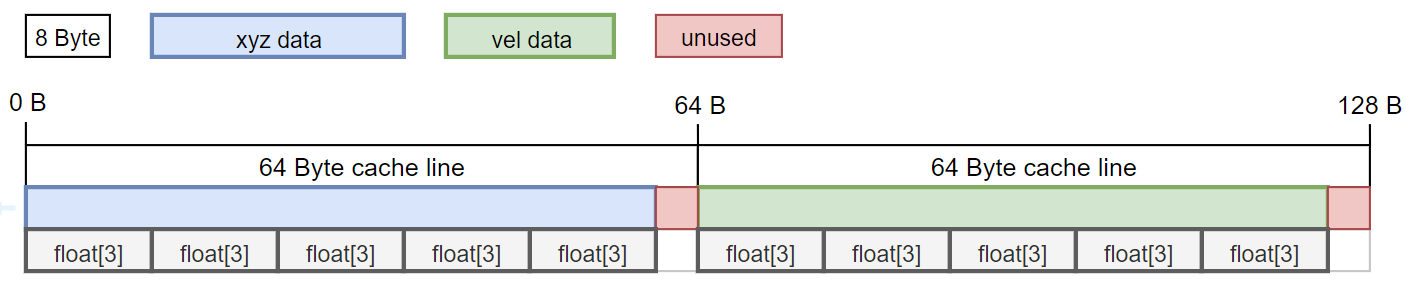
\includegraphics[width=1.0\linewidth, height=0.17\linewidth]{PICs/CacheUtilizationNPCSOA}
	\caption{xyz and vel blocks inside cache-lines, where blue is joint float[3] blocks of xyz data, green is joint blocks of float[3] vel data and red is unused but intentional padding.}\label{cache_utilization_soa}
\end{figure}
\\This leads to consistent throughput. In numbers we now have exactly two cache misses per five \textit{NPCs} (We don't really have an NPC object anymore, but we are still allowed to \textit{think} in objects). One for the positional data, one for the velocity data. Again for 1000 NPCs this would now result in 400 cache misses what translates to $225\times\sim300$ clock cycles less latency than the AOS version, for position updates alone! Each frame!\\\\
This is starting to behave \textit{optimal}. By not loading unneeded data into the cache we can store more relevant data. By Aligning and padding our data blocks correctly we attenuate the chance of \textit{conflict misses} since we reduces the number of cache-lines related data depends on. We do however still have leftover space. The four Byte paddings we append to each $5\times float[3]$ block has purpose, yet could theoretically hold information. Imagine our now theoretical NPC and thus our positional computation would involve a per NPC factor for maybe damping, as well as a mass. Still assuming that $sizeof(float) = 4$ this would be an additional eight Byte per NPC on each computation. Following our SOA approach we would define yet two new arrays for the damping factor and mass respectively. Accessing them would result in the utilization of another two cache-lines. Even though those cache-lines now suffice 16 NPCs each ($\frac{64}{sizeof(float)} = 16$) we now are dependent on four individual cache-lines to compute the \textit{update\_npc\_position} for one NPC, so the amount of cache-lines scales linearly with the amount of parameters the function depends on (for SOA). In terms of eviction and consequently of conflict misses, this could yet again cultivate sub-optimal cache utilization. For the same reasons Intel's article on \textit{Memory Layout Transformations}\mc{aosoa} also mentions increased pressure on the \textit{TLB} (Translation Look-aside Buffer).\\
Even though we reduced the overall NPC per cache-line ratio, there is still unused information and scaling prone to eviction, all due to the individually related data blocks being physically separated. This doesn't countermand that SOA is arguably better than AOS, but it indicates, that there is still room for improvement.

\subsection{Regarding temporal- and spatial locality / Components / AOSOA}\label{rtasl}
The motivation behind our AOS to SOA conversion, was to maximize cache utilization when processing an NPC's position. We figured, that loading an object entails lots of unwanted data that does not share temporal locality with the information that is relevant to us. So we made sure, that instead of objects we loaded only wanted data.
\begin{wrapfigure}[10]{r}{0.4\textwidth}
	\begin{lstlisting}[language=C++,numbers=none,name={Consolidating related data},label={component_npc}]
	struct npc_group{
		float xyz[3];
		float vel[3];
		float mass, damping;
	};
	
	npc_group npc_groups[NUM_ENTITIES];
	\end{lstlisting}
\end{wrapfigure}
In order to do so we gave up something very important. When data is logically related it means, that it collaborates. Whenever we see, that certain subsets of data are frequently used together it is advisable not to separate them. So instead of rigorously converting each member into an array pendant, we group logically related data and create arrays of those groups instead \refcodep{component_npc}.This way the relevant data concerning one NPC will not spread over different incoherent cache-lines, that could map to completely different segments in main memory.\\
This technique bundles related data and makes sure it is successive in memory as well as in cache-lines, consequently we won't peril those cache-lines to extrude each other from the cache. The book \textit{Compilers, Principles, Techniques and Tool} also describes a mechanism like this and refers to those groups as \textit{blocks} \mcp{aho}{786}.
Also we get the chance to fully exploit our hardware's boundaries, as in now we can get rid of manually inserted padding Bytes \reffigp{cache_utilization_comp} - provided we have related data that fits the gap.
\begin{figure}[!htbp]
	\centering
	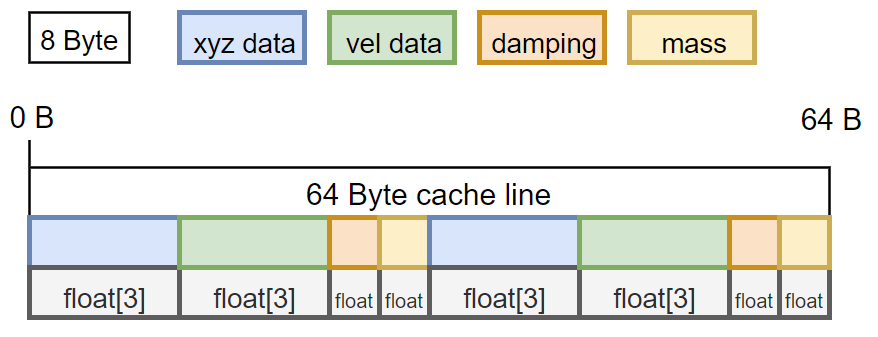
\includegraphics[width=.6\linewidth, height=0.16\linewidth]{PICs/CacheUtilizationNPCComp}
	\caption{unified relevant data in a cache-line.}\label{cache_utilization_comp}
\end{figure}
It is however only possible to gain a performance boost out of this, when the unified data is actually logically related. Whenever data is unified we basically have the same problem, we tried to get rid of in the first place - possibly loading unwanted data into the cache, increasing access latency. The moment we decide, that for example our game should provide the player with an indicator to which NPC is nearest to the player's avatar, we again would be doomed to load adherent information about the NPC's velocity, mass and stuff that was grouped to make position updates faster. Because for this we actually only want the NPCs' positions.
\newpage
\subsubsection{Hot/Cold Splitting}
\begin{wrapfigure}[14]{l}{0.34\textwidth}
\begin{lstlisting}[language=C++,numbers=none,name={The NPC class splitted into hot/cold data},label={hcsplit_npc}]
struct npc_cold_data{
	char *name;
	int age;
	int mood;
};

struct npc{
	float xyz[3];
	float vel[3];
	npc_cold_data *cold_data_ptr;
};
\end{lstlisting}
\end{wrapfigure}
A famous practical application of grouping a particular subset of data is called a \textit{Hot/Cold Split} \mcp{nystrom}{283}. It is also used to improve cache utilization, only it has a very specific definition of what members should be grouped.\\
The idea is to separate a record's member definitions into two subsets. One that contains all the hot-, and one that contains all the cold members, respectively. Data is hot when it is used frequently and cold when it is used rarely \mcp{chilimbi}{8}. By grouping together all the hot data we want to make sure, that data which is frequently used has a higher chance to exist in a cache line on access.\\
The cold data is externalized into a struct of its own. The original struct now contains only the hot data, as well as a pointer to a cold struct instance. Since access frequency does not necessarily resemble the original partitioning of the fields, this pattern emphasizes the preference of logical over contextual relation.\\
Especially for monolithic class definitions, there can be numerous logical subsets of data fields. For example one data subset of a classic OOP gameobject will mainly be used for physics calculations (velocity, acceleration, mass, colliders), another for rendering (vertice data, shaders, textures) and yet another that embeds the game object in the game's environment (health, strength, gold, stamina, etc.).\\
First of all it is not always apparent whether a field is hot/cold. An experienced programmer might feel confident enough for a reasonably small class definition to eyeball it. A better approach might be to wrap our fields with access mechanisms that let us count how often they are accessed at run time, yet again we could rely on static analysis. Since this work will specifically implement a hot/cold split in the prototype we will get back to this in TODO REF SEC.\\
Also we might end up picking individual fields of contextually differing data subsets. We could for example identify \textit{velocity, vertice data, gold} as our hot fields, because they are frequently accessed. However they are utilized at different times of the game and individually they have no common logical relation that is relevant to our computations!\\
Even a split that divides contextual relation might result in a performance boost, if only the cold data is 'cold enough', but just as well a bad split might result in even worse cache utilization.
In order to make a decision, that regards temporal- and spatial locality in a complex situation, we might need to find a way to evaluate, compare and eventually prioritize individual fields. An attempt to solve this will be made in the prototypical implementation, so more on that later on.

\subsubsection{Components}
After a grouping procedure the remnant members of the original NPC class could also be grouped by the same method we talked about before: take related members unify them in a struct and store those structs in an array so they are beyond equals. If the original class hierarchy was designed well the grouping of related data bits will start to resemble it, which might look like a step backwards at first, but remember, the related data groups are packed in seperate single purpose arrays and what counts is the access patterns to retrieve them. When we are done grouping all related data bits of the original NPC object, we will have recreated a so called \textit{component pattern} \mcp{nystrom}{213}.\\
In the classical component pattern we will keep a container object that holds instances of each component \mcp{nystrom}{214}. In favor of performance the container object should only hold pointers to the instances lying in their respective array. But actually and if we were able to group all domains of the original class, the object might be nothing else but an index, that can be used to retrieve a group out of its array.\\
Components are one widely used mechanism to decouple parts of a formerly shared entity. This is applied to classes and is therefore a statement to how OOP and DoD can work hand in hand. Not only is the component pattern useful for decoupling and performance interests, it also solves issues, that would normally be solved by applying multiple inheritance \mcp{nystrom}{215}, which is a practice even despised by OOP enthusiasts.\\
Components can be stored domain wise, while still being contextually linked individually on an object instance level. Their decoupling mechanism have proven great maintainability and even provide a comparably light weight interface for game designers. Accessing them can be done domain wise as well -> optimal cache utilization. This elegant arrangement between OOP and DoD makes it a favored pattern for modern game engines \mcp{fabian}{83}.

\subsubsection{Array Of Structure Of Arrays (AOSOA)}
\begin{wrapfigure}[12]{r}{0.4\textwidth}
\begin{lstlisting}[language=C++,numbers=none,name={AOSOA variant of grouped NPC traits},label={aosoa_npc}]
struct npc_bucket{
	float
	xyz[3] [SUB_SET_SIZE],
	vel[3] [SUB_SET_SIZE],
	mass   [SUB_SET_SIZE],
	damping[SUB_SET_SIZE];
};

npc_bucket npc_buckets[NUM_BUCKETS];
\end{lstlisting}
\end{wrapfigure}
At first glance the idea of reintroducing the AOS concept seems confusing. In some cases depending on the original access patterns it might however be a good idea to separate the total amount of data into chunks that are often referred to as \textit{Buckets}. We already went a step back before, when we decided to unify logically related bits and make arrays of groups. We figured, that this might be an optimal solution for a very specific computation, but might behave poorly in other situations. An attempt is to again separate the relevant members, however to a certain extend gain back the advantage of spatial locality. \textit{The idea here is to get the benefit of locality at the outer-level and also unit-stride at the innermost-level}\mc{aosoa}. Applied to our NPC it might look like \refcode{aosoa_npc}. We merely define our former \textit{columns}/arrays to hold only a subset of the total data respectively. The structure, that holds our member-arrays (the SOA) will however now be emplaced inside an array itself (the AO)! In Other words: We keep the data that will be used to transform each other close to prevent eviction. We enable the user to access specific members individually, to prevent loading unnecessary information.\\
This attempt is compossible with grouping certain members, too. After all we are still able to access only specific sub arrays of buckets. To retain the benefit of \textit{page-locality} for the grouped member-arrays we need to find a fitting \textit{bucket-size : number-buckets} ratio. In case of our \refcode{aosoa_npc} example, taken to the extreme $\textit{NUM\_BUCKETS}=1$ would practically result in the classic SOA model, coming with all its advantages and disadvantages. On the other hand $\textit{SUB\_SET\_SIZE}=1$ would pretty much just be an object definition again (only needlessly more confusing and incomplete since we grouped the members).\\
If we want to optimize against our L1D cache, that performs an 8-way associativity mapping on 64 Byte cache-lines, we could argue that $\frac{8\times 64}{(8\times sizeof(float)} = 16$ might be a fitting \textit{SUB\_SET\_SIZE}, because all the elements in a bucket would then be guaranteed to map to different cache-lines. So no conflict misses when performing transformations on related data groups. Note that this statement is only 100\% valid as long as our buckets are aligned correctly.\\
Finding the NPC next to the player would now mean iterating the \textit{xyz} subsets of each bucket. Depending on the data bundled in a bucket (especially concerning alignment and padding) we still need to expect to load unwanted data subsequently to \textit{xyz} but this will now happen on a \textit{per-bucket} basis rather than on a \textit{per-NPC} basis.
